\documentclass[11pt]{cernrep}
\usepackage{graphicx,epsfig}
\bibliographystyle{lesHouches}


% Packages needed for proceedings
\usepackage{amsmath}
\usepackage{hepunits}
\usepackage[caption=false]{subfig}

% Comments to be commented out when done
\usepackage{color}
\definecolor{darkgreen}{rgb}{0,0.5,0}
\newcommand{\jdt}[1]{\textbf{\textcolor{darkgreen}{(#1 --jdt)}}}
\definecolor{darkblue}{rgb}{0,0,0.5}
\newcommand{\gs}[1]{\textbf{\textcolor{darkblue}{(#1 --gs)}}}

\begin{document}

\section{SYSTEMATICS OF QUARK/GLUON TAGGING\protect\footnote{Section coordinators: Gregory Soyez and Jesse Thaler}$^{,}$\protect\footnote{Contributing authors: Marat Freytsis, Philippe Gras, Deepak Kar, Simon Pl\"atzer, Andrzej Siodmok, Peter Skands, and Davison Soper}$^{,}$\protect\footnote{Additional input: Samuel Bein, Andy Buckley, Jon Butterworth, Mario Campanelli, Andrew Larkoski, Peter Loch, Chris Pollard, Salvatore Rappoccio, Alexander Schmidt, Frank Tackmann, and Wouter Waalewijn}}

By measuring the substructure of a jet, one can assign it a ``quark'' or ``gluon'' tag.  In the eikonal limit, quark/gluon discrimination is determined solely by the color factor of the initiating parton ($C_F$ versus $C_A$).  In this section, we confront the challenges faced when going beyond this leading-order understanding, using both parton shower generators and first-principles calculations to assess the impact of higher-order perturbative and non-perturbative physics.  Working in the idealized context of electron-positron collisions, where there exists an unambiguous definition of quark and gluon jets, we find a fascinating interplay between perturbative shower effects and non-perturbative hadronization effects.

\subsection{Overview}
\label{quarkgluon_sec:overview}

Jets are a robust tool for studying short-distance collisions involving quarks and gluons.  With a suitable jet definition, one can connect jet measurements made on clusters of hadrons to perturbative calculations made on clusters of partons \cite{}.  More ambitiously, one can try to tag jets with a suitably-defined flavor label, thereby enhancing the fraction of, say, quark-tagged jets over gluon-tagged jets.  This is relevant for searches for physics beyond the standard model, where signals of interest are often dominated by quarks while the corresponding backgrounds are dominated by gluons.  A wide variety of quark/gluon discriminants have been proposed \cite{}, and there is a growing catalog of quark/gluon studies at the Large Hadron Collider (LHC) \cite{}.

In order to achieve robust quark/gluon tagging, though, one needs theoretical and experimental control over quark/gluon radiation patterns.  At the level of eikonal partons, a quark radiates proportional to its $C_F = 4/3$ color factor while a gluon radiates proportional to $C_A = 3$.  In this proceedings, we demonstrate that quark/gluon discrimination performance is highly sensitive to subleading perturbative effects beyond the eikonal limit, such as $g \to q \overline{q}$ splittings and color coherence, as well as to non-perturbative effects such as color reconnection and hadronization.   While these effects are modeled (to differing degrees) in parton shower generators, they are relatively unconstrained by existing collider measurements, especially in the gluon channel.  The goal of this proceedings is to highlight these uncertainties, which then suggests a set of future LHC measurements that will improve the modeling of jets in general and quark/gluon tagging in particular.

A common misconception about quark/gluon tagging is that it is an intrinsically ill-defined problem.  Of course, quark and gluon partons carry color while jets are composed of color-singlet hadrons, so the labels ``quark'' and ``gluon'' are fundamentally ambiguous.  But this is philosophically no different from the fact that a ``jet'' is fundamentally ambiguous and one must therefore always specify a concrete jet finding procedure.  As discussed in section~\ref{quarkgluon_sec:def}, the proper way to think about quark/gluon discrimination is in the context of unambiguous hadron-level measurements.  In that sense, quark/gluon tagging is a well-defined technique for enhancing desired signals over undesired backgrounds.

There are a wide range of possible quark/gluon discriminants and a similarly large range of ways to quantify discrimination power.  As a concrete set of discriminants, we consider the generalized angularities $\lambda_\beta^\kappa$ \cite{} at five different $(\kappa, \beta)$ working points, discussed further in section~\ref{quarkgluon_sec:genang}.  These roughly map onto five variables in common use in the literature:
\begin{equation}
\text{multiplicity}, \quad p_T^D, \quad \text{LHA}, \quad \text{width}, \quad \text{mass},
\end{equation}
where LHA refers to the ``Les Houches Angularity'', named after the workshop of this proceedings.  To quantify discrimination performance, we focus on classifier separation \cite{}:
\begin{equation}
\Delta =  \frac{1}{2} \int \text{d} \lambda \, \frac{\bigl(p_q(\lambda) - p_g(\lambda)\bigr)^2}{p_q(\lambda) + p_g(\lambda)},
\end{equation}
where $p_q$ ($p_g$) is the probability distribution for a quark-tagged (gluon-tagged) sample.

We begin our parton shower generator predictions in section~\ref{quarkgluon_sec:ee}, using idealized case of quark/gluon discrimination in $e^+e^-$ collisions.  Here, we can use the following processes as unambiguous proxies for quark and gluon jets:
\begin{align}
\text{``quark jets''}: \quad & e^+e^- \to (\gamma/Z)^* \to u \overline{u}, \\
\text{``gluon jets''}: \quad & e^+e^- \to h^* \to g g.
\end{align}
These processes are physically distinguishable by the quantum numbers of the associated color singlet production operator, giving a way to label quarks and gluons without reference to the final state.  We compare four different parton shower generators, not only at their default configurations but also with physically-motivated changes:
\begin{itemize}
\item \textsc{Pythia 8.205} \cite{}
\item \textsc{Vincia 1.201} \cite{}
\item \textsc{Herwig++ 2.7.1} \cite{}
\item \textsc{Sherpa 2.1.1} \cite{}
\end{itemize}
As we will see, the dominant differences between programs arise from physics at the interface between perturbative showering and non-perturbative fragmentation.   \jdt{I AM HERE}  In section~\ref{quarkgluon_sec:ee_scales} section~\ref{quarkgluon_sec:ee_settings}.

\jdt{This needs to be rewritten}In section~\ref{quarkgluon_sec:pp}, we suggest a possible analysis strategy at the LHC to constrain quark/gluon radiation patterns.  At a hadron collider, the distinction between quark jets and gluon jets is rather subtle, since radiation patterns depend on color connections between the measured final state jets and the unmeasured initial state partons.  That said, we find that one can already learn a lot from hadron-level measurements, without trying to isolate ``pure'' quark or gluon samples.  In particular, we advocate measuring the generalized angularities on quark/gluon enriched samples:
\begin{align}
\text{``quark enriched''}: \quad & pp \to W/Z/\gamma + \text{jet}, \\
\text{``gluon enriched''}: \quad & pp \to \text{dijets},
\end{align}
where ``enriched'' means that the Born-level process contributing to these channels is dominated by the corresponding jet flavor.  For completeness, we also study the gluon-enriched process $pp \to H + \rm{jet}$; even though this process has a relatively small cross section at the LHC, it is a useful benchmark for our Monte Carlo comparisons.  By making judicious kinematic cuts, we could further flavor-enrich these samples \cite{}, though we will not pursue that in this paper for simplicity.

We present our final recommendations and conclusions in section~\ref{quarkgluon_sec:conclude}.  The main take home message from this study is that, contrary to the standard lore, measurements at $e^+e^-$ colliders are insufficient to constrain uncertainties in the final state shower.   Therefore, gluon-enriched measurements at the LHC will be crucial to constrain final state radiation patterns.

\subsection{What is a Quark/Gluon Jet?}
\label{quarkgluon_sec:def}

As part of the 2015 Les Houches workshop on ``Physics at TeV Colliders'', an attempt was made to define exactly what is meant by a ``quark jet'' or ``gluon jet''.  Here are some suggested options for defining a quark jet, in order from most ill-defined to most well-defined.

\noindent \textbf{A quark jet is...}
\begin{itemize}
\item \textbf{A quark parton.}  This definition (incorrectly) assumes that there is a one-to-one map between a jet and its initiating parton.  Because it neglects the important role of additional radiation in determining the structure of a jet, we immediately dismiss this definition.
\item \textbf{A Born-level quark parton.}  This definition at least acknowledges the importance of radiative corrections to jet production, but leaves open the question of how exactly to define the underlying Born-level process from an observed final state.  For one answer, see flavored jet algorithms below.
\item \textbf{The initiating quark parton in a final state parton shower.}  We suspect that this is the definition most LHC experimentalists have in mind.  This is sometime referred to as the ``max-$p_T$'' prescription \cite{}, though it assumes that the parton shower history is meaningful, which may not be the case beyond the strongly-ordered or leading-logarithmic approximations.  Because the parton shower is semi-classical, this definition neglects the impact of genuinely quantum radiative corrections as well as non-perturbative hadronization. 
\item \textbf{An eikonal line with baryon number 1/3 and carrying triplet color charge.}  This is another semi-classical definition that attempts to use a well-defined limit of QCD to define a quark in terms of light-like Wilson lines.  Philosophically, this is similar to the parton shower picture, with a similar concern about how to extrapolate this definition away from the strict eikonal limit.
\item \textbf{A parton-level jet object that has been quark-tagged using an infrared and collinear (IRC) safe flavored jet algorithm.}  This is the strategy adopted in \cite{} (see also \cite{}).  While this definition neglects the impact of hadronization, it does allow for the calculation of quark jet cross sections at all perturbative orders, including quantum corrections.
\end{itemize}
The unifying theme in the above definitions is that they are trying to identify a quark as an object unto itself, without reference to the specific final state of interest.  However, it is well-known that a ``quark'' in one process may not look like a ``quark'' in other process, due to color correlations with the rest of the event, especially the initial state in $pp$ collisions.  The next definition attempts to deal with the process dependence in defining quarks. 
\begin{itemize}
\item \textbf{A quark operator appearing in a hard matrix element in the context of a factorization theorem.}  This is similar to the attitude taken in \cite{}.  In the context of a well-defined cross section measurement, one can (sometimes) go to a limit of phase space where the hard production of short-distance quarks and gluons factorizes from the subsequent long-distance fragmentation.  This gives quarks a nice (gauge-covariant) operator definition of a quark jet.  That said, even if a factorization theorem does exist for the measurement of interest, this definition is potentially ambiguous beyond leading power.
\end{itemize}
The definition we adopt in this paper is inspired by the idea that one should always think about quark tagging in the context of a specific measurement, but it tries to avoid relying on the presence of a factorization theorem.
\begin{itemize}
\item \textbf{A phase space region (as defined by an unambiguous hadronic fiducial cross section measurement) that yields an enriched sample of quarks (as interpreted by some suitable, though fundamentally ambiguous, criterion).}  Here, the goal is to \emph{tag} a phase space region as being quark-like, rather than try to determine a truth definition of a quark.  This definition has the advantage of being explicitly tied to hadronic final states and to the discriminant variables of interest.   Of course, the main challenge with this definition is how to determine the criterion that corresponds to successful quark-enrichment.  For that, we will have to rely to some degree on the other less well-defined notions of what a quark jet is.
\end{itemize}  

It is worth emphasizing that this last definition separates the measurement process from the interpretation process.  That is, one first measures hadron-level discriminant variables on a final state of interest, and only later does one interpret exactly what that discrimination accomplishes (either as quark/gluon separation or as some more sophisticated classification).  Ultimately, we will be recommending that the LHC experiments perform measurements of the generalized angularities $\lambda_\beta^\kappa$ in well-defined hadron-level final states.  It is then a separate interpretation step to infer something about parton-level quark/gluon radiation patterns from these hadron-level measurements.

\subsection{Generalized Angularities}
\label{quarkgluon_sec:genang}

\begin{figure}
\centering
\subfloat{
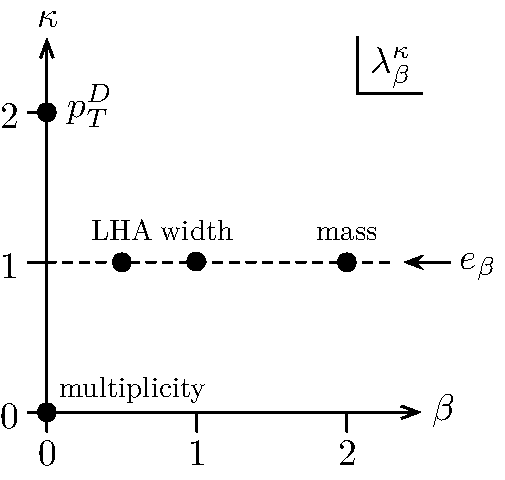
\includegraphics[scale = 0.7]{quarkgluon_fig_lambda_space.pdf}
}
\caption{Two parameter family of generalized angularities, adapted from \cite{Larkoski:2014pca}.  The dots correspond to the five benchmark angularities used in our study.}
\label{fig:lambda_space}
\end{figure}

A wide variety of quark/gluon discriminants have been proposed (see \cite{} for a catalog), but here we limit ourselves to a two-parameter family of generalized angularities \cite{}, shown in figure~\ref{quarkgluon_fig:lambda_space}.  These are defined as
\begin{equation}
\label{eq:genang}
\lambda^{\kappa}_{\beta} = \sum_{i \in \text{jet}} z_i^\kappa \theta_i^\beta,
\end{equation}
where $i$ runs over the jet constituents, $z_i \in [0,1]$ is a momentum fraction, and $\theta_i \in [0,1]$ is a (normalized) recoil-free angle. The parameters $\kappa \ge 0$ and $\beta \ge 0$ determine the momentum and angle weighting, respectively.  For $\kappa = 1$, the generalized angularities are IRC safe and hence calculable in perturbation theory \cite{}, and we will sometimes use the shorthand
\begin{equation}
e_\beta \equiv \lambda^{1}_{\beta}. 
\end{equation}
There are also techniques to treat the $\kappa \not= 1$ case using generalized fragmentation functions \cite{Larkoski:2014pca}.  In our Monte Carlo studies, we determine $\lambda^{\kappa}_{\beta}$ using all constituents of a jet, though one could also consider using charged-particle-only angularities to improve robustness to pileup.

For our $e^+ e^-$ study, we cluster jets using the $ee$-variant of the anti-$k_t$ algorithm \cite{}, with $|\vec{p}|$-ordered winner-take-all recombination \cite{} to determine the jet axis $\hat{n}$.  Note that unlike in standard $E$-scheme recombination, the jet axis $\hat{n}$ is not necessarily aligned with the jet momentum $\vec{p}$, which turns out to be a desirable feature for avoiding soft recoil effects \cite{}.  We then define
\begin{equation}
z_i \equiv \frac{E_i}{E_{\rm jet}}, \qquad \theta_i \equiv \frac{\Omega_{i \hat{n}}}{R},
\end{equation}
where $\Omega_{i \hat{n}}$ is the opening angle to the jet axis and $R$ is the jet radius (taken to be $R = 0.6$ by default).  For our $pp$ study, we use the standard $pp$ version of anti-$k_t$, with $p_T$-ordered winner-take-all recombination, defining
\begin{equation}
z_i \equiv \frac{p_{Ti}}{\sum_{j \in \text{jet}} p_{Tj}}, \qquad \theta_i \equiv \frac{R_{i \hat{n}}}{R},
\end{equation}
where $R_{i \hat{n}}$ is the rapidity-azimuth distance to the jet axis.

By adjusting $\kappa$ and $\beta$, one can probe different aspects of the jet fragmentation.  We consider five benchmark values for $(\kappa, \beta)$ indicated by dots in figure~\ref{quarkgluon_fig:lambda_space}:
\begin{equation}
\label{eq:benchmarkang}
\begin{aligned}
(0,0) &= \text{particle multiplicity},\\
(2,0) &\Rightarrow p_T^D \text{  \cite{} (specifically $\lambda^{2}_{0} = (p_T^D)^2$)},\\
(1,0.5) & = \text{Les Houches Angularity (LHA)},\\
(1,1) &= \text{width or broadening \cite{}} ,\\
(1,2) & \Rightarrow \text{mass or thrust \cite{} (specifically $\lambda^{1}_{2} \simeq m_{\rm jet}^2 / p_{T{\rm jet}}$)}.
\end{aligned}
\end{equation}
Except for the LHA, these angularities (or their close cousins) have already been used in quark/gluon discrimination studies.  The LHA has been included to have an IRC safe angularity that weights energies more heavily than angles, similar in spirit to the $\beta = 0.2$ value advocated in ref.~\cite{}.

For the IRC safe case of $\kappa = 1$, there is an alternative version
of the angularities based on energy correlation functions \jdt{not
  sure about my definition here, especially factors of 2.}\gs{I
  usually define this without the $1/2$ and normalised by $1/R^\beta$}
\begin{equation}
\text{ecf}_\beta = \frac{1}{2}\sum_{i \not= j \in \text{jet}} z_i z_j \theta_{ij}^\beta \simeq \lambda^{1}_{\beta},
\end{equation}
where equality holds in the extreme eikonal limit.\footnote{This equality also relies on using a recoil-free axis choice $\hat{n}$ to define $\theta_i$.}  Amusingly, $\lim_{\beta \to 0} \text{ecf}_\beta = 1 - 2  \lambda^{2}_{0}$ \cite{} (i.e.~$\kappa = 2$, $\beta = 0$).  To avoid a proliferation of curves, we will not show any results for $\text{ecf}_\beta$.  We will also neglect quark/gluon discriminants that take into account azimuthal asymmetries within the jet, such as elliptically \cite{} and 2-subjettiness \cite{}, though azimuthal information can improve quark/gluon discrimination \cite{}.

\subsection{Quantifying Quark/Gluon Separation Power}
\label{quarkgluon_sec:ee}

\jdt{This needs to be rewritten, with footnote on mutual information}Since we will be testing many Monte Carlo variants, we need a way to quantify quark/gluon separation power in a robust way that can easily be summarized by a single number.  For that purpose we use classifier separation \cite{}:
\begin{equation}
\Delta =  \frac{1}{2} \int \text{d} \lambda \, \frac{\bigl(p_q(\lambda) - p_g(\lambda)\bigr)^2}{p_q(\lambda) + p_g(\lambda)},
\end{equation}
where $p_q$ ($p_g$) is the probability distribution for the quark-tagged (gluon-tagged) sample.  Here, $\Delta = 0$ corresponds to no discrimination power and $\Delta = 1$ corresponds to perfect discrimination power.  Because $\Delta$ is defined as an integral, one can use standard error propagation to assign statistical uncertainties on the Monte Carlo results.


To demonstrate the importance of final state evolution, we begin our quark/gluon studies with the idealized case of discriminating $e^+ e^- \to (\gamma/Z)^* \to u \bar{u}$ (quark-tagged) from $e^+ e^- \to h^* \to gg$ (gluon-tagged).  Here, the flavor of the outgoing jets is fixed by the Lorentz structure of the production vertex.  Of course, even in the quark-tagged sample, there can be ``gluon jets'', as in $e^+ e^- \to u \bar{u} g$ where a hard gluon recoils against a nearly collinear $u \bar{u}$.  This reflects the intrinsic ambiguity in the definition of jet flavor.   To resolve that ambiguity, we rely on the production vertex alone to define the truth-level jet flavor.

\begin{figure}
\centering
\subfloat[]{
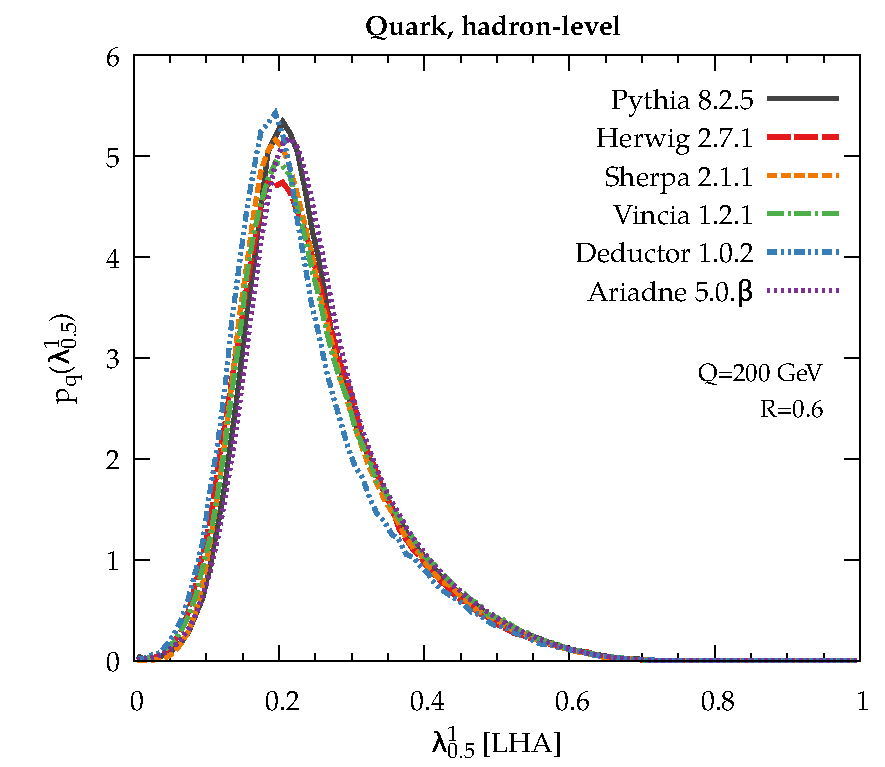
\includegraphics[width = 0.45\columnwidth]{quarkgluon_fig_GA_10_05_R6_hadron_quark.pdf}
\label{fig:LHA_hadron_quark}
}
$\quad$
\subfloat[]{
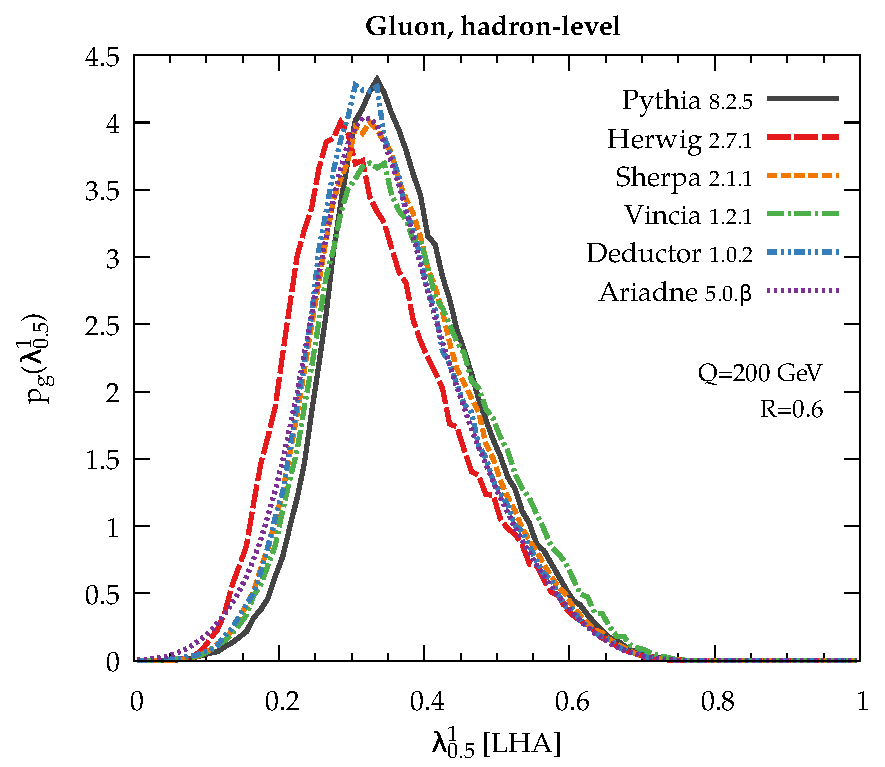
\includegraphics[width = 0.45\columnwidth]{quarkgluon_fig_GA_10_05_R6_hadron_gluon.pdf}
\label{fig:LHA_hadron_gluon}
}
$\quad$
\subfloat[]{
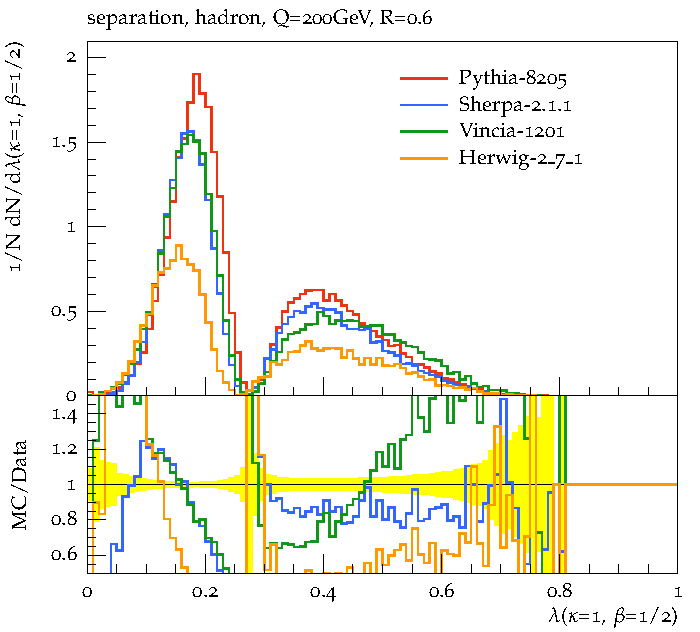
\includegraphics[width = 0.45\columnwidth]{quarkgluon_fig_GA_10_05_R6_hadron_separation.pdf}
\label{fig:LHA_hadron_separation}
}
\caption{Distributions of the LHA for (a) the $e^+ e^- \to u \bar{u}$ quark-tagged sample, (b) the $e^+ e^- \to gg$ gluon-tagged sample, and (c) the classifier separation integrand in Eq.~\eqref{eq:deltaintegrand}.  All four parton shower generators are run at their baseline settings.  \jdt{Is there a way to make the font size bigger in the yoda plots?}}
\label{fig:LHA_hadron}
\end{figure}


In figure~\ref{quarkgluon_fig:LHA_hadron} we show distributions of the LHA (i.e.~$e_{0.5}$) in the quark sample ($p_q$) and gluon sample ($p_g$), comparing the baseline settings of four different parton shower generators at a center-of-mass collision energy of $Q = 200~\GeV$ with jet radius $R = 0.6$. In the quark sample, there is relatively little variation between the generators, which is not surprising since all four programs have been tuned to match LEP data (though LEP never measured the LHA itself).  There are somewhat larger variations between the generators in the gluon sample, since there is no data to directly constrain $e^+ e^- \to gg$.  We also see qualitative agreement of the analytic calculations with the parton shower results, though not quantitative agreement; this will be discussed further in section~\ref{quarkgluon_subsec:testingshape} below.  


In figure~\ref{quarkgluon_fig:LHA_hadron_separation}, we plot the integrand of classifier separation:
\begin{equation}
\label{eq:deltaintegrand}
\frac{1}{2} \frac{\bigl(p_q - p_g\bigr)^2}{p_q + p_g}.
\end{equation}
This quantity shows where in the LHA phase space the actual discrimination power lies, with large values of the integrand corresponding to places where the quark and gluon distributions are most dissimilar.  Now we see considerable differences between the generators, reproducing the well-known fact that \textsc{Pythia} is more optimistic about quark/gluon separation while \textsc{Herwig} is more pessimistic.

\begin{figure}
\centering
\subfloat{
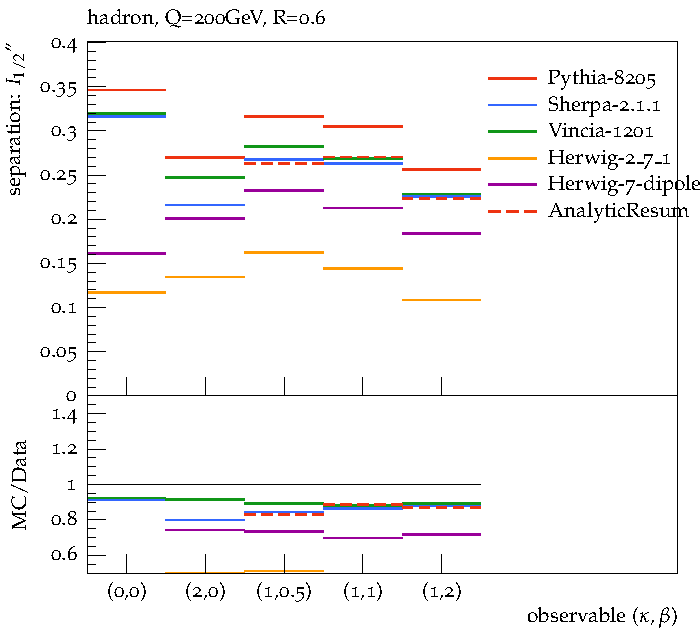
\includegraphics[width = 0.45\columnwidth]{quarkgluon_fig_I2_R6_hadron__all.pdf}
}
\caption{Classifier separation for the five different benchmark angularities, determined from four different parton shower generators.}
\label{fig:summary_hadron_all}
\end{figure}

To summarize the overall discrimination power, we integrate Eq.~\eqref{eq:deltaintegrand} to obtain the value of $\Delta$ for the LHA.  This is shown in figure~\ref{quarkgluon_fig:summary_hadron_all}, which also includes the four other benchmark angularities from Eq.~\eqref{eq:benchmarkang}.  There is a rather large spread in predicted discrimination power between the generators.  While such differences might be expected for IRC unsafe angularities which depend on non-perturbative modeling, these differences persist even for the IRC safe angularities, indicating a more fundamental difference between the generators that is already present at parton level.  In the rest of this section, we explore these differences in order to ascertain their origin.

\subsection{Parameter Dependence}
\label{quarkgluon_sec:ee_scales}

Given the large absolute differences in discrimination power, we next want to check if the four generators exhibit similar or dissimilar trends as parameters are varied.  We perform three parameter sweeps, using the bolded values below as defaults:
\begin{equation}
\begin{aligned}
\text{Collision Energy}: Q &= \{ 50, 100, \mathbf{200}, 400, 800\}~\GeV, \\
\text{Jet Radius}: R &= \{ 0.2, 0.4, \mathbf{0.6}, 0.8, 1.0\}, \\
\text{Strong Coupling}: \alpha_s / \alpha_{s0} &= \{0.8,0.9,\mathbf{1.0},1.1,1.2\}, \\
\end{aligned}
\end{equation}
where $\alpha_{s0}$ is the default value of the coupling, which is different between generators (and sometimes different between different aspects of the same generator).

The resulting values of $\Delta$ are shown in figure~\ref{quarkgluon_fig:ee_sweep}, which not only shows hadron-level results, but also parton-level results where the hadronization step in each program has been turned off.  For the analytic results, parton-level results do not include the non-perturbative shape function.   There are number of surprising features in these plots.  First, even for the IRC safe angularities, the effect of hadronization is rather large, both on the absolute scale of discrimination and the trends.  Second, the slope of the trends can flip signs between different generators.  \jdt{More discussion.  Need to understand why analytic calculations go in wrong direction sometimes.}

\begin{figure}
\centering
\subfloat[]{
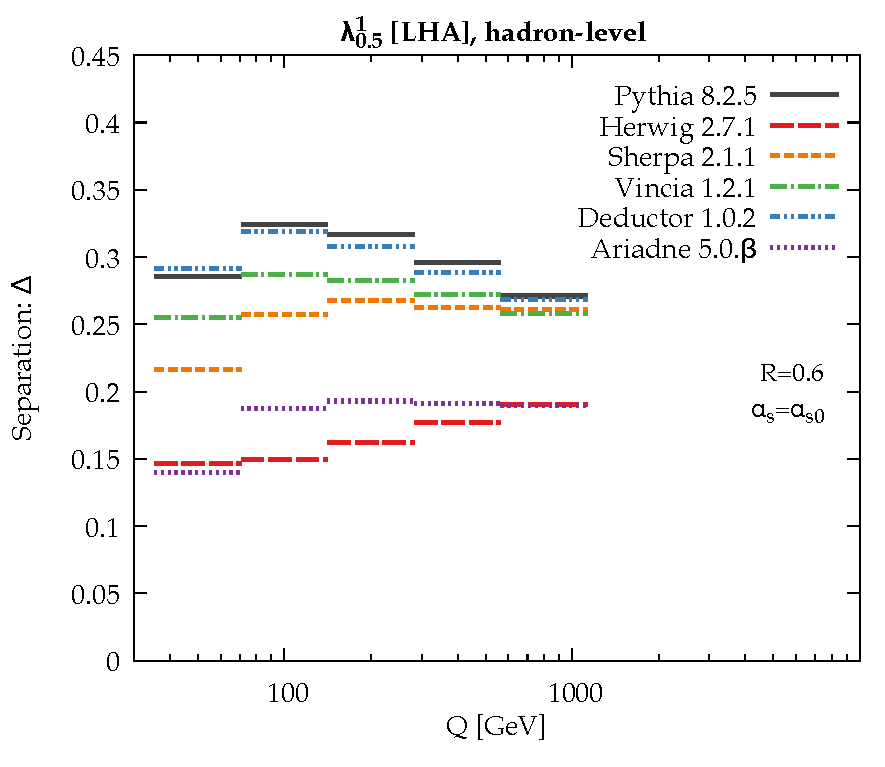
\includegraphics[width = 0.4\columnwidth]{quarkgluon_fig_I2_GA_10_05_hadron_Qdep.pdf}
\label{fig:sweep_Q_hadron}
}
$\quad$
\subfloat[]{
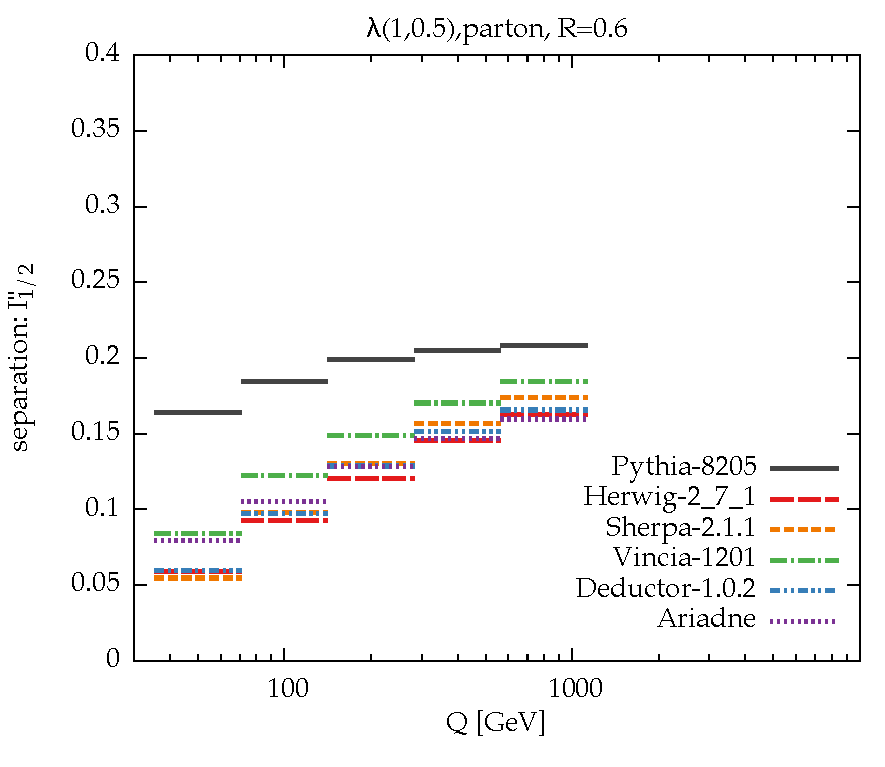
\includegraphics[width = 0.4\columnwidth]{quarkgluon_fig_I2_GA_10_05_parton_Qdep.pdf}
\label{fig:sweep_Q_parton}
}
$\quad$
\subfloat[]{
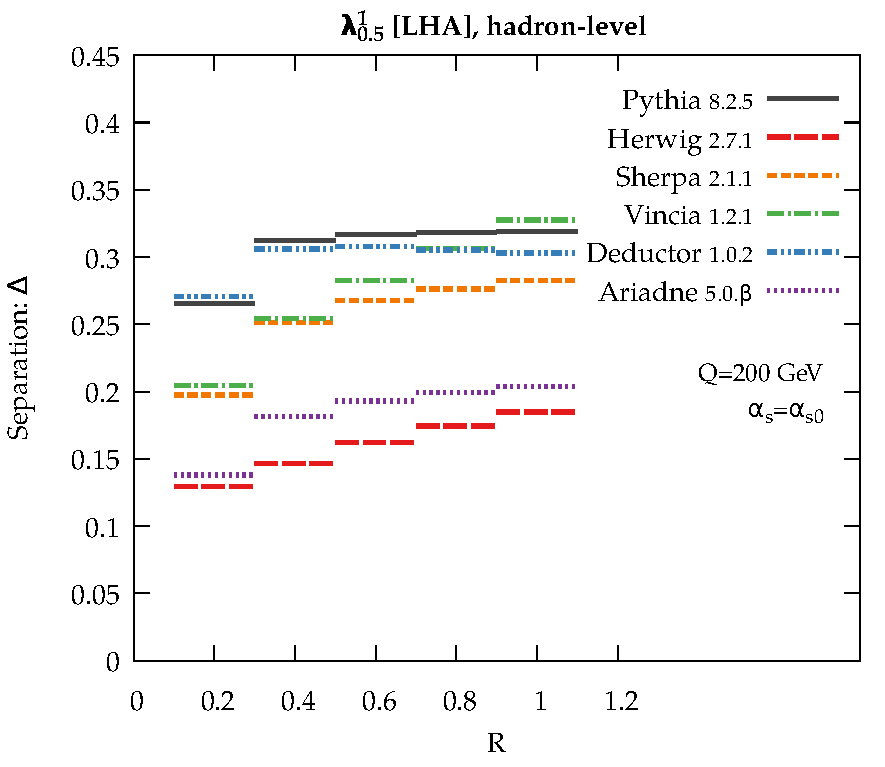
\includegraphics[width = 0.4\columnwidth]{quarkgluon_fig_I2_GA_10_05_hadron_Rdep.pdf}
\label{fig:sweep_R_hadron}
}
$\quad$
\subfloat[]{
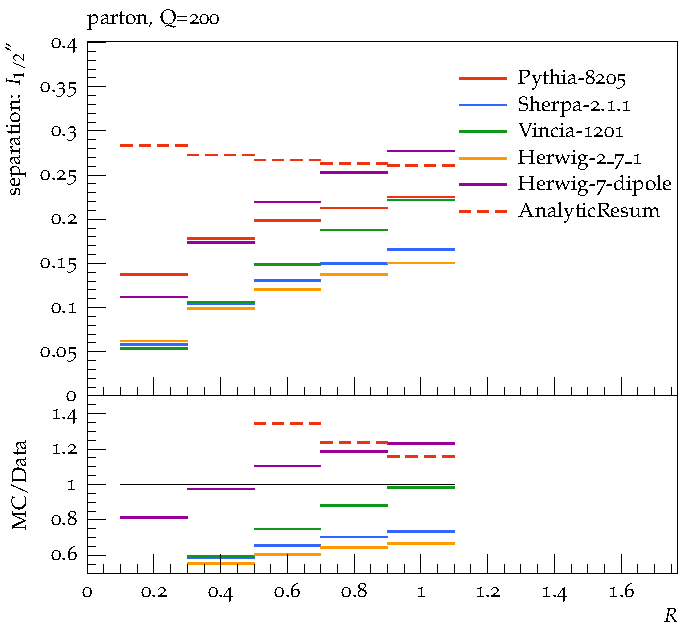
\includegraphics[width = 0.4\columnwidth]{quarkgluon_fig_I2_GA_10_05_parton_Rdep.pdf}
\label{fig:sweep_R_parton}
}
$\quad$
\subfloat[]{
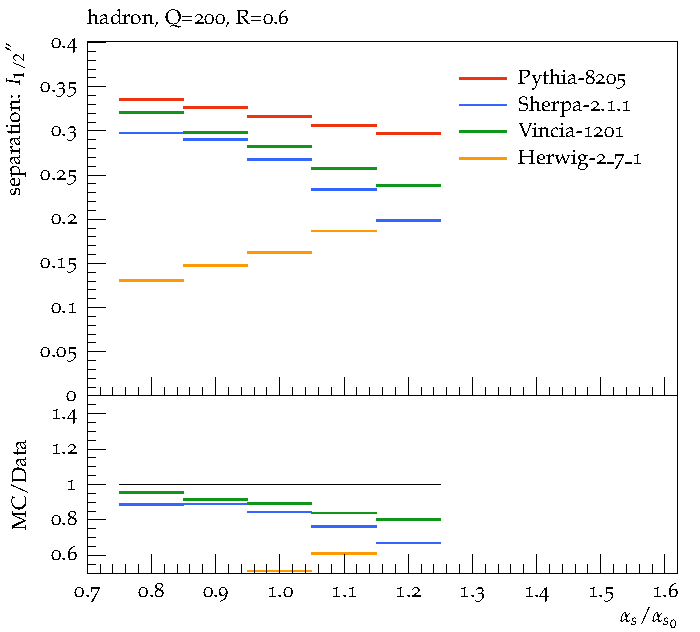
\includegraphics[width = 0.4\columnwidth]{quarkgluon_fig_I2_GA_10_05_hadron_alphadep.pdf}
\label{fig:sweep_as_hadron}
}
$\quad$
\subfloat[]{
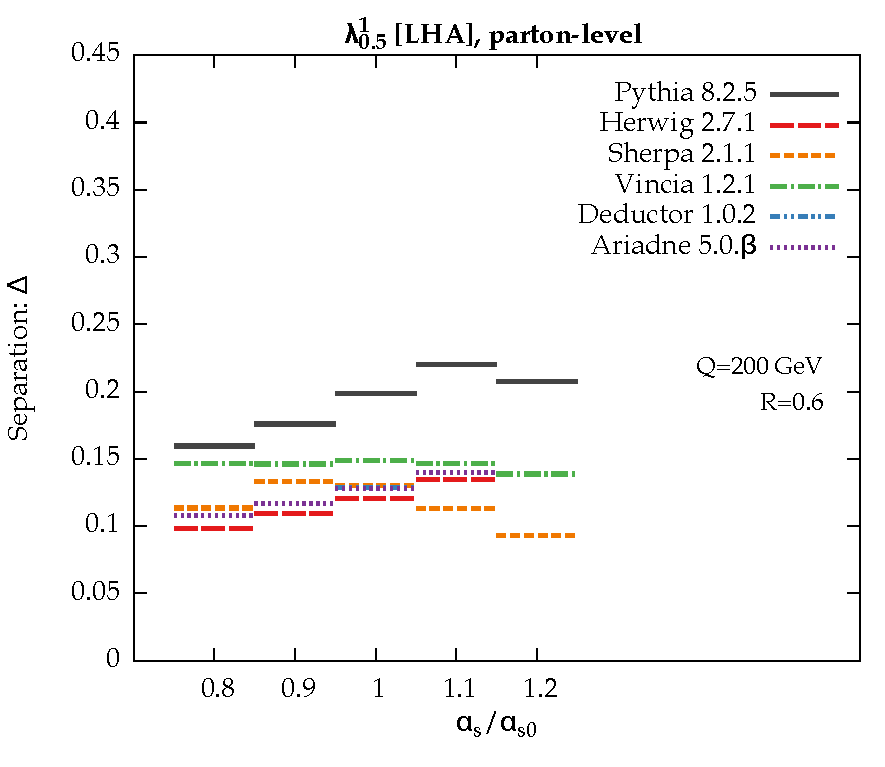
\includegraphics[width = 0.4\columnwidth]{quarkgluon_fig_I2_GA_10_05_parton_alphadep.pdf}
\label{fig:sweep_as_parton}
}
\caption{Sweeping the collision energy $Q$ (top row), jet radius $R$ (middle row), and coupling constant $\alpha_s/\alpha_{s0}$ (bottom row).  Results are shown at hadron level (left column) as well as at parton level (right column).  \jdt{Is this for LHA or some other variable?}}
\label{fig:ee_sweep}
\end{figure}

\subsection{Impact of Generator Settings}
\label{quarkgluon_sec:ee_settings}

\begin{figure}
\centering
\subfloat[]{
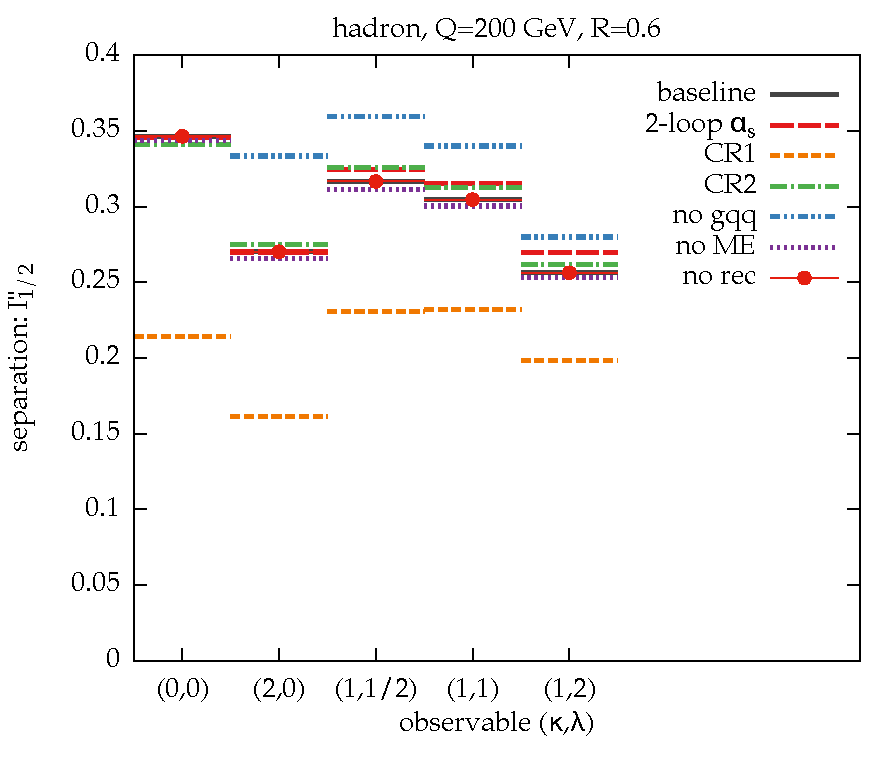
\includegraphics[width = 0.45\columnwidth]{quarkgluon_fig_I2_R6_hadron_pythia.pdf}
\label{fig:summary_hadron_pythia}
}
$\quad$
\subfloat[]{
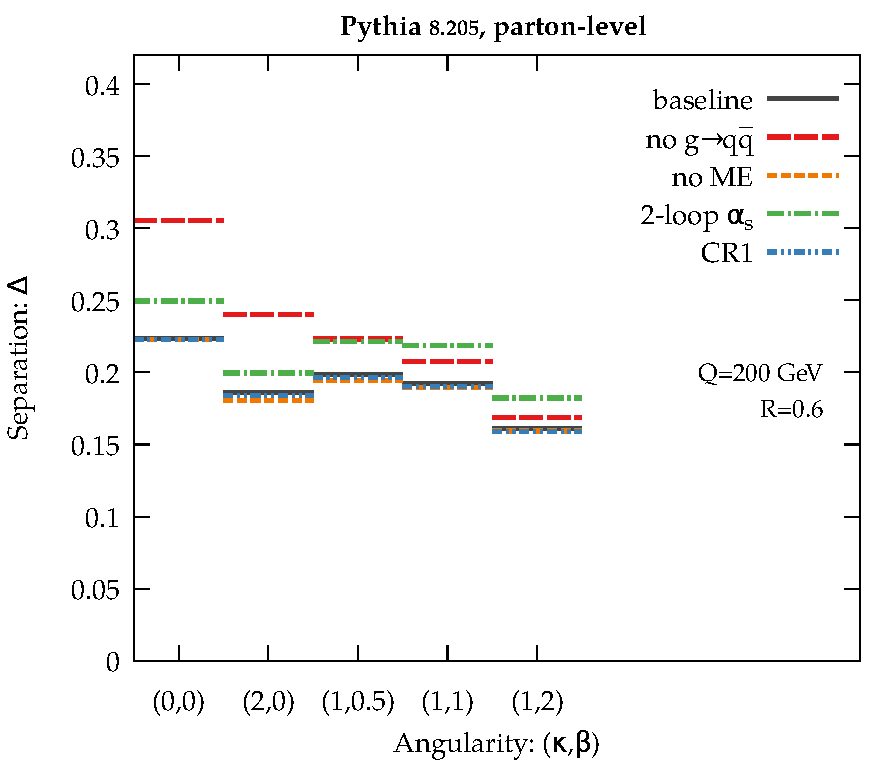
\includegraphics[width = 0.45\columnwidth]{quarkgluon_fig_I2_R6_parton_pythia.pdf}
\label{fig:summary_parton_pythia}
}
$\quad$
\subfloat[]{
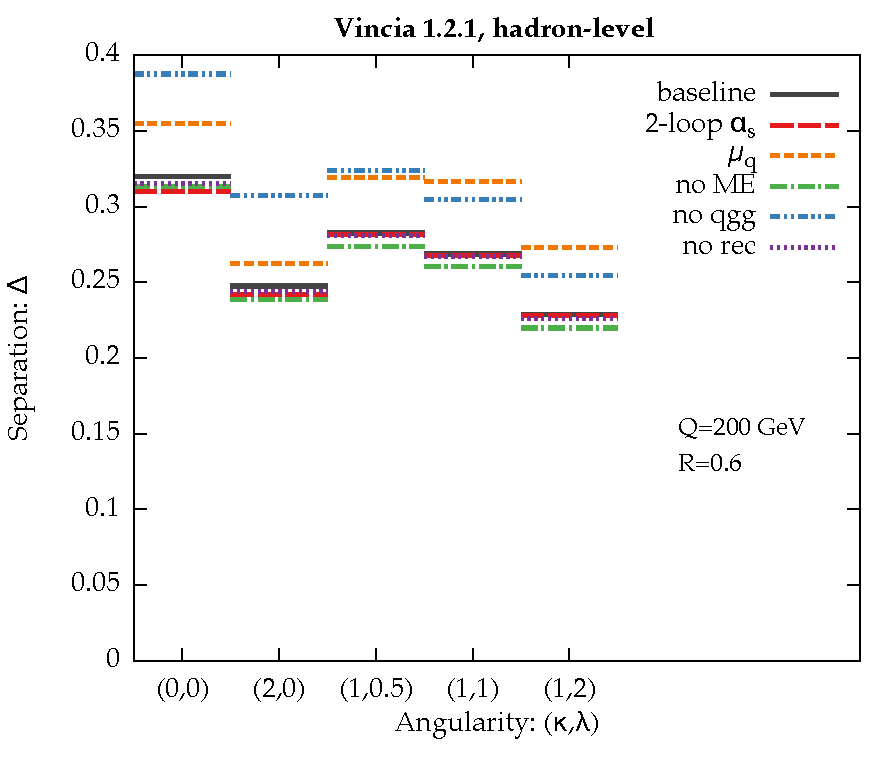
\includegraphics[width = 0.45\columnwidth]{quarkgluon_fig_I2_R6_hadron_vincia.pdf}
\label{fig:summary_hadron_vincia}
}
$\quad$
\subfloat[]{
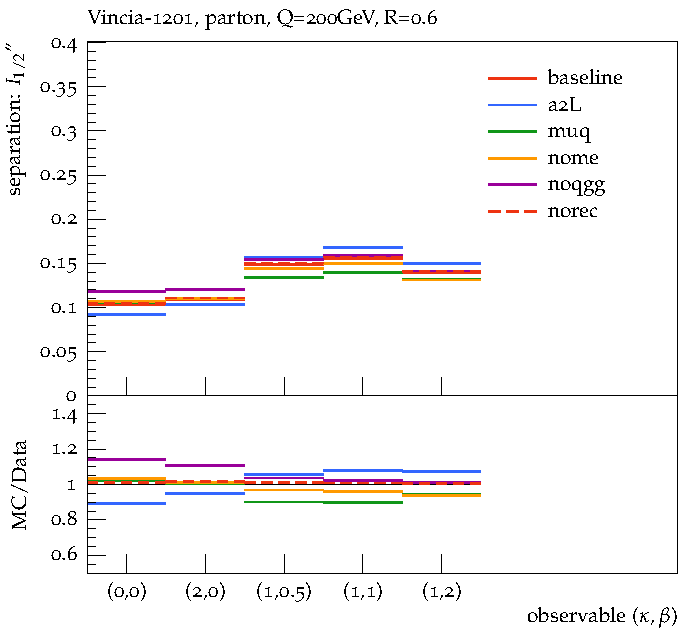
\includegraphics[width = 0.45\columnwidth]{quarkgluon_fig_I2_R6_parton_vincia.pdf}
\label{fig:summary_parton_vincia}
}
\caption{Settings variants in \textsc{Pythia} (top row) and \textsc{Vincia} (bottom row).  Shown are hadron-level results (left column) and parton-level results (right column).}
\label{fig:settings_variation_1}
\end{figure}

\begin{figure}
\centering
\subfloat[]{
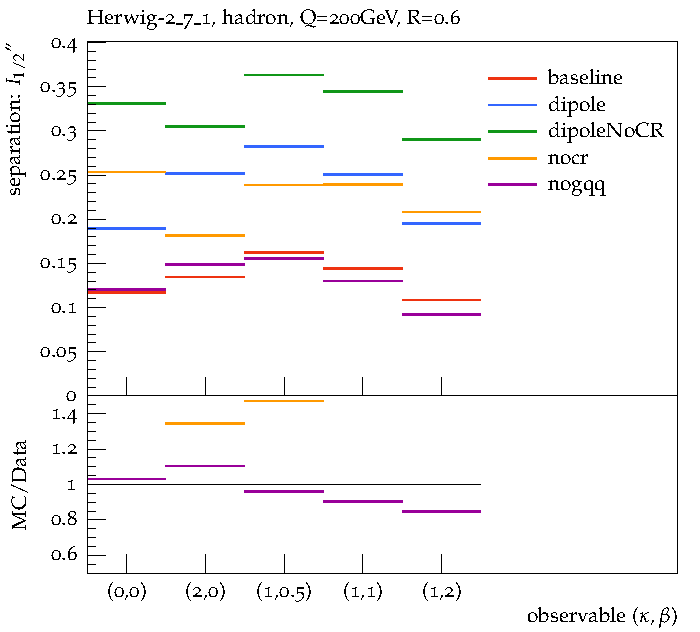
\includegraphics[width = 0.45\columnwidth]{quarkgluon_fig_I2_R6_hadron_herwig.pdf}
\label{fig:summary_hadron_herwig}
}
$\quad$
\subfloat[]{
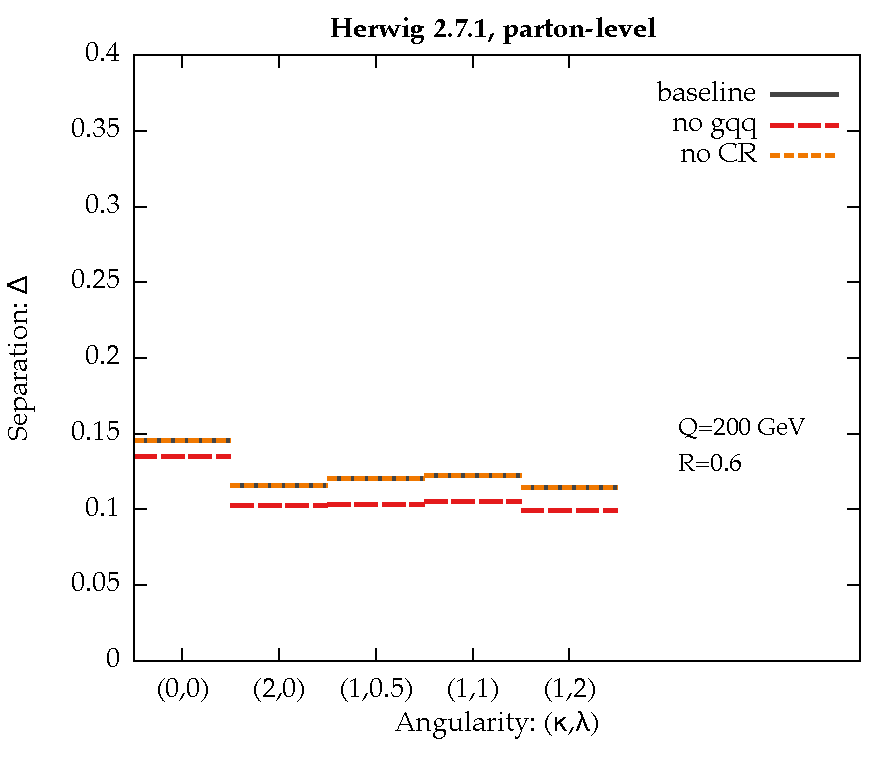
\includegraphics[width = 0.45\columnwidth]{quarkgluon_fig_I2_R6_parton_herwig.pdf}
\label{fig:summary_parton_herwig}
}
$\quad$
\subfloat[]{
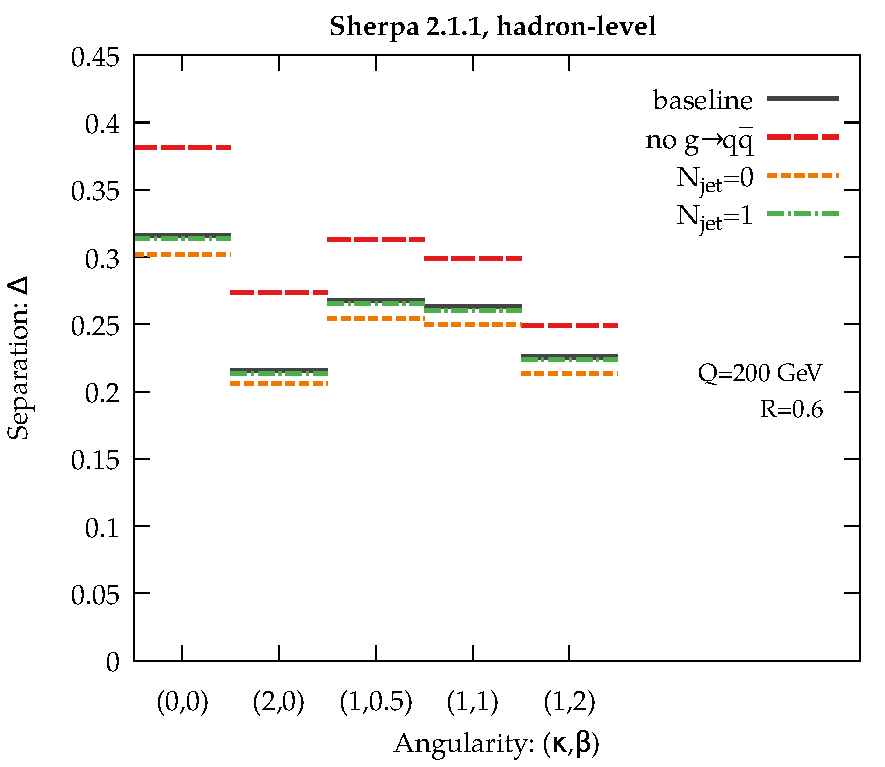
\includegraphics[width = 0.45\columnwidth]{quarkgluon_fig_I2_R6_hadron_sherpa.pdf}
\label{fig:summary_hadron_sherpa}
}
$\quad$
\subfloat[]{
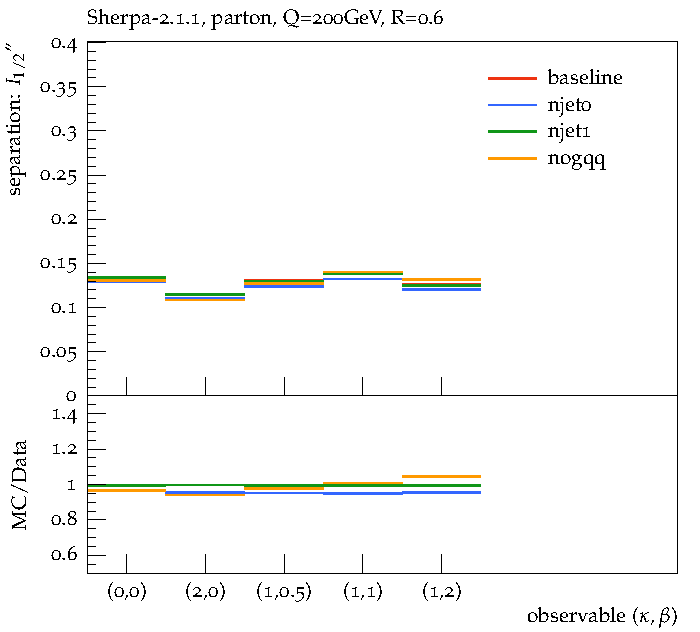
\includegraphics[width = 0.45\columnwidth]{quarkgluon_fig_I2_R6_parton_sherpa.pdf}
\label{fig:summary_parton_sherpa}
}
\caption{Same as figure~\ref{quarkgluon_fig:settings_variation_1}, but for (top row) \textsc{Herwig} and (bottom row) \textsc{Sherpa}.}
\end{figure}


\begin{figure}
\centering
\subfloat[]{
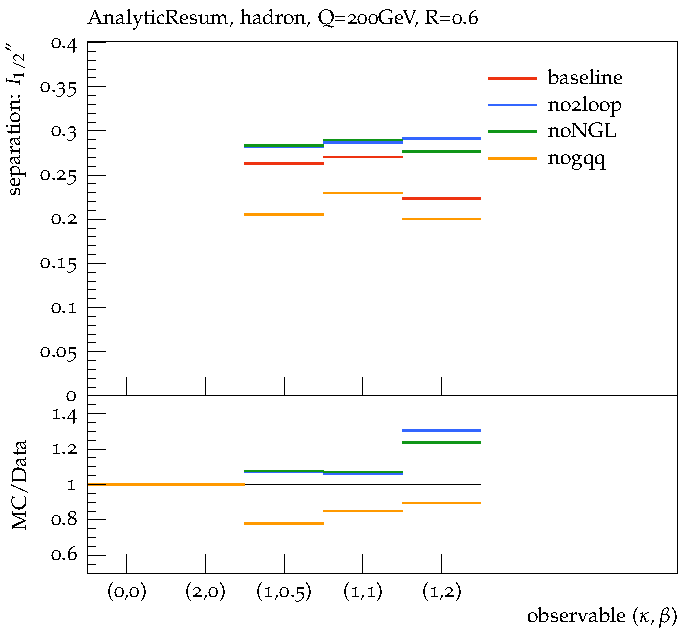
\includegraphics[width = 0.45\columnwidth]{quarkgluon_fig_I2_R6_hadron_analytic.pdf}
\label{fig:summary_hadron_analytic}
}
$\quad$
\subfloat[]{
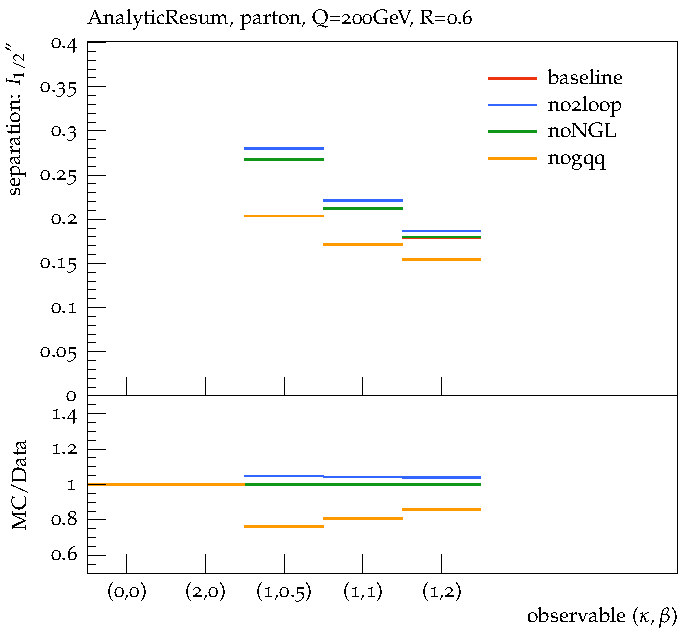
\includegraphics[width = 0.45\columnwidth]{quarkgluon_fig_I2_R6_parton_analytic.pdf}
\label{fig:summary_parton_analytic}
}
\caption{Same as figure~\ref{quarkgluon_fig:settings_variation_1}, but for the analytic calculation.}
\end{figure}



Formally, parton shower generators are only accurate to modified leading logarithmic (MLL) accuracy, though they include physically important effects like energy/momentum conservation and matrix element corrections that go beyond MLL.  We now assess the impact of these higher-order effects by changing the baseline parameter settings in each of the generators.

\jdt{We should split into hadron-level and parton-level settings changes.}


\begin{itemize}
\item \textsc{Pythia} : CR1, CR2, a2L, nogqq, nome, norec
\item \textsc{Vincia} : a2L, muq, nome, nogqq, norec
\item \textsc{Herwig} : dipole, dipoleNoCR, nocr, nogqq
\item \textsc{Sherpa} : njeto0, njet1-noqq, njet1
\end{itemize}

\subsection{Looking Towards the LHC}
\label{quarkgluon_sec:pp}

It is clear from our $e^+e^-$ study that quark/gluon radiation patterns are not under good theoretical control, even accounting only for final state physics effects.  Beyond just the application to quark/gluon tagging, this is an important challenge for any analysis that uses jets.  In order to resolve these issues and improve parton shower modeling of jets, measurements from the LHC will be essential (as will improved analytic calculations).  In this section, we perform an example analysis for $pp$ collisions that highlights the kind of information one can gain about quark/gluon radiation patterns, despite the additional complications faced by hadronic collisions.

\begin{figure}
\centering
\subfloat{
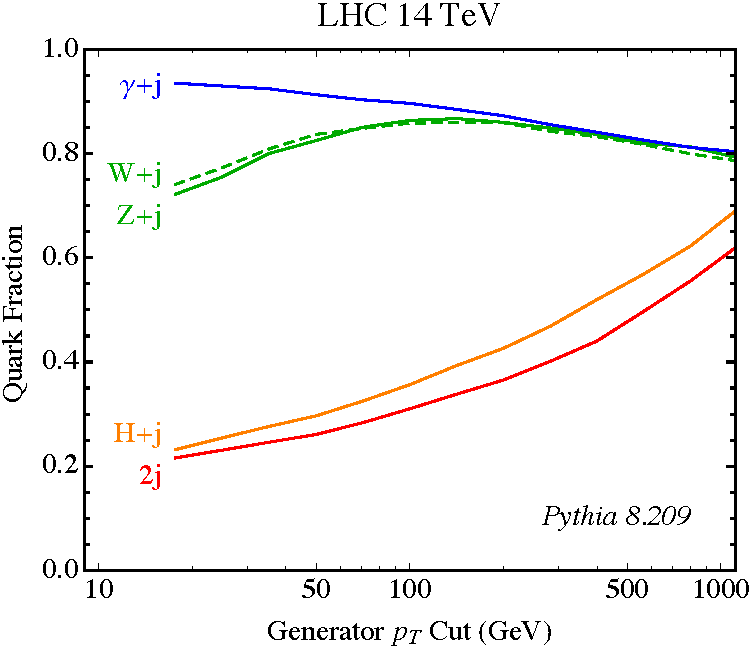
\includegraphics[width = 0.45\columnwidth]{quarkgluon_fig_parton_level_qg_composition.pdf}
}
\caption{Quark fraction of jets at parton level, as defined by the generator-level parton flavor.}
\label{fig:parton_level_qg_composition}
\end{figure}

There is no way to isolate pure samples of quark or gluon jets at the LHC, but we can isolate quark/gluon-enriched samples, as defined by the flavor label of the jet in the corresponding Born-level partonic process.  As shown in figure~\ref{quarkgluon_fig:parton_level_qg_composition}, the Born-level jet in $W/Z/\gamma + \text{jet}$ is more than 70\% quark enriched over the entire jet $p_T$ range of interest.  For jets softer than around 200 GeV, the Born-level jet in dijets or $H+\text{jet}$ is more than 60\% gluon enriched, with that fraction decreasing as the jet $p_T$ increases.  In principle, could could try to ``diagonalize" some combination of vector boson plus jet and dijet samples in order to define separate quark or gluon samples (see \cite{}).  In this study, we will simply ask the question whether one can tell ``the jets in $Z$ plus jet" (quark-enriched) apart from "the jets in dijets" (gluon-enriched).  

In figure~\ref{quarkgluon_}, we show LHA distributions for quark-enriched and gluon-enriched samples.  \jdt{Need plot to say more.}

\subsection{Summary and Recommendations}
\label{quarkgluon_sec:conclude}

By measuring the substructure of jets, it is possible to gain information about the quark/gluon composition of a jet sample.  The challenge we have identified in this paper is that the precise radiation pattern of quark and gluon jets is poorly understood, in the sense that parton shower generators give rather different predictions for absolute quark/gluon discrimination power as well as relative trends as a function of the jet kinematics.  At the moment, analytic calculations are not at a level of accuracy where they can offer any useful guide.  Therefore, LHC data is the best hope to constrain quark/gluon radiation patterns and enable quark/gluon discrimination to be a robust tool.

In terms of specific measurements that should be highest priority for ATLAS and CMS, our study has not revealed a silver bullet.  \jdt{Still true in pp with grooming?}  Rather, all of the generalized angularities studies showed similar levels of disagreement between generators, so a systematic LHC study of even one observable is likely to offer crucial new information.  What is essential is to make measurements at multiple jet $p_T$ scales and multiple jet radii $R$.  Unfolded distributions would likely be most useful for parton shower tuning, but even detector-level measurements compared to detector-simulated parton showers would help spot troubling trends.

The key lesson to parton shower authors is that LEP data \emph{does not} constrain all of the relevant aspects of the final state parton shower.  While we have extensive information about quark jet radiation patterns, gluon jet radiation patterns are essentially unconstrained.  This has important implications for parton shower tuning strategies.  Specific recommendations:
\begin{itemize}
\item \textit{Gluon splitting to quarks}:  Some of the largest difference between generators came from turning on and off the $g \to q \overline{q}$ process.  \jdt{...}
\item \textit{Color reconnection in the final state}:  Color reconnection is usually thought of as an issue mainly at hadron colliders.  \jdt{...}
\item \textit{Reconsidering $\alpha_s$ defaults}:  \jdt{...}
\end{itemize}



\bibliography{quarkgluon_bib}

\end{document}
